\lab{Importance Sampling}{Importance Sampling}
\objective{Though Monte Carlo integration is a useful strategy for estimating integrals, the standard implementation suffers slow convergence and can be inaccurate.
This typically occurs when the domain of integration is very small, making it unlikely that very many, if any, randomly chosen points will lie inside of it.
Importance sampling remedies this problem by choosing the sample points more intelligently.
This situation happens most frequently when trying to approximate integrals of probability distributions, so we focus on integrating common probability density functions.}

\section*{Monte Carlo Simulation} % ===========================================

The standard procedure of Monte Carlo integration is not always the most efficient or accurate way to estimate an integral.
Consider the probability density function (p.d.f) of the standard normal distribution in one dimension,
\begin{equation}
f_X(t) = \frac{e^{-t^2/2}}{\sqrt{2\pi}}.
\label{eq:imsamp-standard-normal}
\end{equation}
The probability that a random draw from the standard normal distribution is greater than $3$ is given by the integral
\begin{equation}
\int_{3}^{\infty} f_X(t)\,dt = \frac{1}{\sqrt{2\pi}}\int_{3}^{\infty} e^{-t^2/2}\:dt.
\label{eq:importsamp-integral}
\end{equation}

If $h: \mathbb{R} \rightarrow \mathbb{R}$ is the indicator function defined by
\[
h(t) = \begin{cases}
1 & \text{ if } t > 3 \\
0 & \text{ if } t \leq 3,
\end{cases}
\]
then \eqref{eq:importsamp-integral} can be rewritten as
\begin{equation}
\int_{3}^{\infty} f_X(t)\:dt = \int_{-\infty}^{\infty} h(t)f_X(t)\:dt.
\label{eq:infinity_integral}
\end{equation}
Note that this process can be generalized to any domain of integration by redefining the indicator function $h$ to match different bounds of integration.

We can now easily estimate this same probability using Monte Carlo simulation.
Given a random collection of draws $\{x_i\}_{i=1}^N$ from the standard normal distribution, we can estimate the integral from \eqref{eq:infinity_integral} as
\begin{equation}
\int_{-\infty}^{\infty} h(t)f_X(t)\,dt \approx \frac{1}{N}\sum_{i = 1}^{N}h(x_i).
\label{eq:importsamp-estimator}
\end{equation}
% Now that the estimator is defined, it is quite manageable to approximate \eqref{eq:importsamp-integral}.
% The estimate will get closer and closer to the actual value as more and more sample points are used.

\section*{Statistics with SciPy} % ============================================
The \li{scipy.stats} module has many features for probability and statistics.
One of the most effective uses of \li{scipy.stats} is to create an object for a particular distribution with the following methods:

\begin{table}[H]
\centering
\begin{tabular}{r|l}
    Method & Description\\
    \hline
    \li{cdf()} & Calculate the cumulative probability evaluated up to a point.\\
    \li{pdf()} & Calculate the probability of drawing a number from a distribution.\\
    \li{rvs()} & Draw a random number from the distribution.\\
\end{tabular}
% \caption{Some methods available for a distribution from scipy.stats.}
\end{table}

The following code shows how to appropriately use the methods of \li{stats} objects.
\begin{lstlisting}
>>> from scipy import stats
>>> import numpy as np

# Create an object for the standard normal distribution.
>>> F = stats.norm()
# loc is the mean and scale is the standard deviation.
>>> G = stats.norm(loc=3, scale=2)

# Calculate the probability of drawing a 1 from the normal distribution.
>>> F.pdf(1)
0.24197072451914337

# Draw a number at random from the normal distribution.
>>> F.rvs()
0.95779975

# Specifying a size returns a numpy.ndarray.
>>> F.rvs(size=2)
array([-0.40375954, 1.10956538])

\end{lstlisting}

Use \li{np.linspace()} and \li{pdf()} in order to plot a distribution.
\begin{lstlisting}
>>> from matplotlib import pyplot as plt
# Create a linspace for our graph.
>>> X = np.linspace(-4, 4, 100)
# Use the normal distribution created previously.
>>> plt.plot(X, F.pdf(X))
>>> plt.show()
\end{lstlisting}

\begin{table}[H]
\centering
\begin{tabular}{r|l}
    Object & Description\\
    \hline
    \li{norm()} & The normal distribution.\\
    \li{gamma()} & The gamma distribution.\\
    \li{multivariate_normal()} & The normal distribution in higher dimensions.\\
    \li{beta()} & The beta distribution.
\end{tabular}
% \caption{Some methods from scipy.stats.}
\end{table}

% See Appendix \ref{appendix:stats-prob-tools} for a more thorough treatment of \li{scipy.stats}.

\begin{problem}
\label{prob:importsamp-mc}
Write a function that accepts an integer parameter $N$.
Use \eqref{eq:importsamp-estimator} to estimate the probability that a random draw from the standard normal distribution is greater than $3$ using $N$ samples.
Return the approximation.
Your answer should approach 0.0013499 for sufficiently large samples.
\end{problem}

In Monte Carlo integration, each random point that is in the region of interest (in this case a number greater than $3$) increases the approximation, and each random point that is not in that region decreases the approximation.
If draws in the region of interest are unlikely, then it is possible that no random draws end up within the region of interest.
The Monte Carlo integration method returns an approximation of $0$ for the integral in this case, which isn't ideal.
So, while standard Monte Carlo integration can get the job done if enough points are used, getting a good approximation requires an unacceptably large number of sample points.

\section*{Importance Sampling} % ==============================================

Importance sampling makes Monte Carlo integration more efficient in circumstances where random draws within the region of interest are unlikely.
Note that in Monte Carlo integration, random points that are close to and within the bounds of integration are more likely to influence the approximation than points that are farther away.
We call these closer points \emph{important} points.
In importance sampling, we call the distribution of the integral we want to estimate the \emph{target distribution}, and we usually denote it $f_X$.
The idea of importance sampling is to choose a new distribution, called the \emph{importance distribution}, that generates more important points.
The importance distribution is usually denoted $g_Y$.
We then modify \eqref{eq:importsamp-estimator} to take advantage of the importance distribution:
\begin{equation} \label{eq:importsamp-importance}
\int_{-\infty}^{\infty} h(t)f_X(t)\,dt \approx \frac{1}{N}\sum_{i = 1}^{N}\frac{h(y_i)f_X(y_i)}{g_Y(y_i)}.
\end{equation}

The fraction $\frac{f_X}{g_Y}$ is called the \emph{importance weight}.
Because of this result, we can use samples $y_1, \cdots , y_N$ from any distribution with equation $g_Y$ to estimate the integral of $f_X$, as long as we multiply $h(y_i)$ by the importance weight.
Note that if the importance distribution is chosen to be the same as the target distribution, or in other words, if we draw from the same distribution we are trying to estimate, then $g_Y = f_X$ and the importance weight is 1.
In this case, the importance sampling method reduces to the original Monte Carlo simulation given by \eqref{eq:importsamp-estimator}.

\begin{figure}[H]
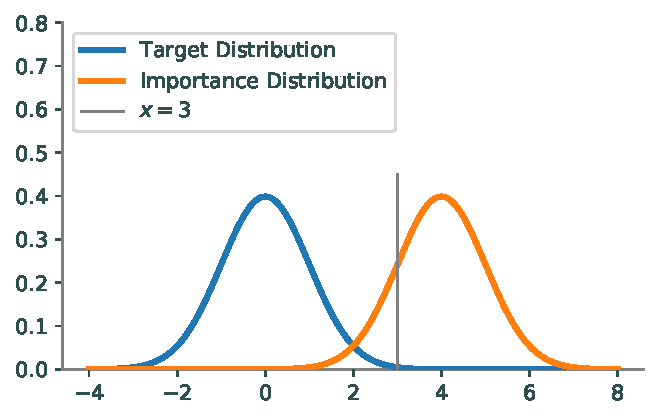
\includegraphics[width=.7\textwidth]{figures/importance_distribution.pdf}
\caption{In our problem, we choose an importance distribution that will generate more samples that are greater than 3. Though not a perfect choice, choosing a normal distribution with $\mu = 4$ and $\sigma = 1$ will suffice.}
\label{fig:importance}
\end{figure}

\begin{info}
The derivation of \eqref{eq:importsamp-importance} is based heavily on the \emph{Law of the Unconscious Statistician}, an important idea in statistics.
See the Additional Materials section for details.
\end{info}

\subsection*{Choosing the Importance Distribution} % --------------------------

There is no correct choice for the importance distribution.
It may be possible to find the distribution that allows the simulation to converge the fastest, but oftentimes, the perfect answer is unnecessary.
Close to perfect is good enough.

To solve the same problem as in Problem \ref{prob:importsamp-mc} using importance sampling, we choose a distribution that will generate more samples close to and greater than 3.
We will choose $g_Y$ to be the normal distribution with mean $\mu = 4$ and standard deviation $\sigma = 1$.
Note that it is not necessary to choose an importance distribution of the same type as the target distribution.

Figure \ref{fig:importance} shows that a random draw from the importance distribution is far more likely to produce a number greater than 3 than a random draw from the target distribution.
However, a draw greater than 3 from the importance distribution is accompanied by a low importance weight because it is so unlikely in the target distribution.
Similarly, a draw less than 3 from the importance distribution has a higher importance weight because it is more likely in the target distribution.

\begin{problem} \label{prob:importsamp-mc_important}
Write a function that accepts a function handle $f$, representing the equation for the target distribution, a function handle $g$, representing the equation for the importance distribution, an indicator function $h$, a function that samples from the importance distribution, and an integer $n$ representing the number of samples to use.
Use \eqref{eq:importsamp-importance} to approximate the integral of the target distribution and return this approximation.

To test your function, estimate the same integral as in Problem \ref{prob:importsamp-mc} using importance sampling.
Choose the importance distribution to be a normal distribution with mean $\mu = 4$ and standard deviation $\sigma = 1$ as shown below.
Your answer should approach $0.0013499$ for large samples.
When compared to Problem \ref{prob:importsamp-mc} this should give more consistent results.

\begin{lstlisting}
# Choose the importance distribution with mean 4 and std dev 1
>>> G = stats.norm(loc=4, scale=1)
>>> g = G.pdf                   # Equation for importance distribution
>>> sampler = G.rvs             # Samples from importance distribution
\end{lstlisting}

\end{problem}

\begin{problem} \label{prob:importsamp-mc_is_compare}
Using the two previous problems, create a plot that compares the error of the traditional method of Monte Carlo integration to the error of the importance sampling method.
Choose your target distribution to be the standard normal distribution, and estimate the probability that a random draw is greater than $3$.
Choose your importance distribution to be the same one you used to test Problem \ref{prob:importsamp-mc_important}.
You should calculate the errors for $n = 5000, 10000, \ldots , 500000$.
Your plot should resemble the following figure.

\begin{figure}[H]
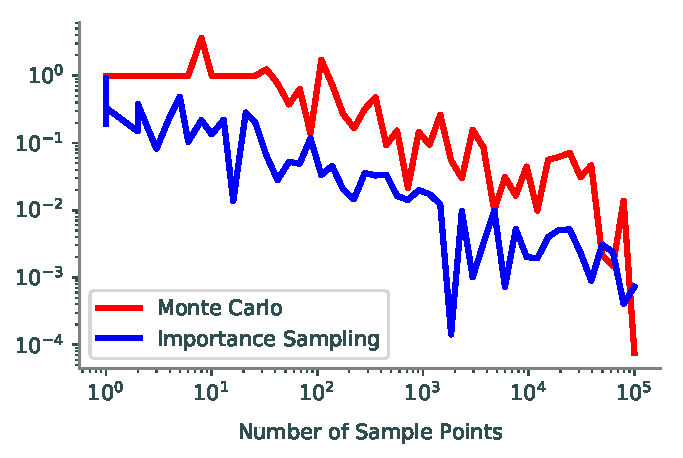
\includegraphics[width=.7\textwidth]{figures/MCvsIS.pdf}
\label{fig:compare}
\end{figure}

To determine the error of your approximations, the following code returns the actual value of the probability:
\begin{lstlisting}
>>> 1 - stats.norm.cdf(3)
\end{lstlisting}
\end{problem}

Problem \ref{prob:importsamp-mc_is_compare} shows that we can achieve the same results as traditional Monte Carlo with only a fraction of the samples if we choose an appropriate importance distribution.
However, even though there is no correct choice for an importance distribution, there are choices that do not give a better approximation of an integral than the Monte Carlo method would without importance sampling.
In Problem \ref{prob:importsamp-mc_important}, we chose a normal distribution with $\mu = 4$ and $\sigma = 1$ to be our importance distribution to test the function.
This produces more points larger than $3$ to use for our integral estimation.
If we had chosen a normal distribution that was less likely to produce points larger than $3$, say for example a normal distribution with $\mu = 0$ and $\sigma = .5$, importance sampling would actually give a larger error than the traditional Monte Carlo method would alone.
In addition, if we had chosen a normal distribution that produced hardly any points less than $3$, the approximation using importance sampling would also be worse.
We examine this further in the next problem.

\begin{problem} \label{prob:other_plots}
Importance Sampling is only as good as the choice of $g_Y$.
Repeat the previous problem of plotting the error for the estimates that a random draw from the standard normal distribution is greater than 3.
Do this for various $g_Y$ by creating 4 subplots.
Each plot displays the error for traditional Monte Carlo as well as the errors of importance sampling for a specific $g_Y$.
Each plot has a different $g_Y$, which will change the importance sampling error.
In all cases let $g_Y$ be a normal distribution with $\sigma =1$, but let $\mu = -1, .25, 4, 7$.
\end{problem}

\section*{Generalizing the Principles of Importance Sampling} % ===============

Up to this point, the target distributions and the importance distributions have all been normal distributions.
Importance sampling works for other types of distributions as well, and even works when the target distribution and the importance distribution are different from each other.
The following problem is an example of this, and gives a potential real world application for importance sampling.

\begin{problem}
\label{prob:importsamp-gamma}
A tech support hotline receives an average of 2 calls per minute.
What is the probability that they will have to wait at least 10 minutes to receive 9 calls?
This problem can be modeled using a gamma distribution.
The equation for calculating the probability of the gamma distribution is
\begin{align}
f_X(x) = \frac{x^{a-1}e^{-x/\theta}}{\Gamma(a)\theta^a}.
\end{align}
Here $a$ is the number of calls we are waiting to receive, $\theta$ is the number of minutes it takes on average to receive one call, and $x$ is the number of minutes needed to wait to receive $a$ calls given $\theta$ calls per minute.
In the above problem, we have $a = 9$, $\theta = .5$, and we want the probability that $x \geq 10$.
Creating the gamma distribution object in \li{scipy.stats} is similar to creating the normal distribution object.
It has the same methods as the normal distribution object.

\begin{lstlisting}
# Create the gamma distribution object with a = 9, theta = .5
>>> F = stats.gamma(a=9, scale=.5)
\end{lstlisting}

Write a function that estimates and returns the probability of having to wait at least $10$ minutes to receive $9$ calls.
Use a normal distribution with mean and standard deviation of your choosing as the importance distribution.
Choose a large enough number of sample points so that the integral is estimated accurately.
Your answer should approach $0.00208726$.
\end{problem}

In addition to single variable distributions, importance sampling can be used to approximate integrals of multivariate functions.
The joint normal distribution of $N$ independent random variables with mean $\0$ and covariance matrix $I$ is
\[
f_X(\x) = \frac{1}{\sqrt{(2 \pi)^N}} e^{-(\x^T\x)/2}.
\]
The integral of $f_X(\x)$ over a box is the probability that a draw from the distribution will be in the box.
However, $f_X(\x)$ does not have a symbolic antiderivative.
Importance sampling can be used here to efficiently estimate the integral of this function.
In the multivariate case, the importance distribution must also be multivariate.
The multivariate normal distribution object in \li{scipy.stats} accepts a mean vector and a covariance matrix as parameters.
The \li{pdf} and \li{rvs} methods work the same as in the single variable case, except that \li{pdf} accepts an array of size $N$ and \li{rvs} returns an array of size $n$ x $N$, where $n$ is the number of samples to draw.
\begin{lstlisting}
# Create a 2-dim multivariate normal object with a zero vector mean and cov matrix I
>>> F = stats.multivariate_normal(mean=np.zeros(2), cov=np.eye(2))
>>> F.pdf(np.array([1,1]))
0.058549831524319168
>>> F.rvs(size=3)
array([[ 0.03429396,  0.13618787],
       [-0.12011818,  0,88691591],
       [-0.16356289,  0.53757853]])
\end{lstlisting}

\begin{problem}
Write a function that estimates and returns the probability that a given random variable in $\mathbb{R}^2$ generated by $f_X$ will be less than -1 in the x-direction and greater than 1 in the y-direction.
Treat $f_X$ as the equation of your target distribution.
Create your own multivariate normal distribution with mean and covariance matrix of your choosing to serve as your importance distribution.
As in the previous problem, choose a large enough number of sample points so that the integral is estimated accurately.
Your answer should approach $0.02517149$.

Hint: The indicator function may have to be coded differently from previous problems to accommodate for the fact that the sampler for the multivariate normal distribution returns a two dimensional array.
Remember that when given an array of samples, the indicator function needs to return either a $0$ or a $1$ for each sample in the array.
\end{problem}

\newpage
\section*{Additional Material}

\subsection*{Derivation of the importance sampling estimator}

By the Law of the Unconscious Statistician (see Volume 2 \S 3.5), we can restate the integral from \eqref{eq:importsamp-integral} as

$$\int_{-\infty}^{\infty} h(t)f_X(t)\,dt = E[h(X)].$$

Then we have

\begin{align*}
E[h(X)] & = \int_{-\infty}^{\infty} h(t)f_X(t)\,dt \\
& = \int_{-\infty}^{\infty} h(t)f_X(t)\left ( \frac{g_Y(t)}{g_Y(t)} \right )\,dt \\
& = \int_{-\infty}^{\infty} \left ( \frac{h(t)f_X(t)}{g_Y(t)} \right )g_Y(t)\,dt \\
& = E\left[\frac{h(Y)f_X(Y)}{g_Y(Y)}\right],
\end{align*}
and the corresponding estimator is

\begin{align*}
\widehat{E}[h(X)] & = \widehat{E}\left [ \frac{h(Y)f_X(Y)}{g_Y(Y)}\right ] \\
& = \frac{1}{N}\sum_{i = 1}^{N}\frac{h(y_i)f_X(y_i)}{g_Y(y_i)}.
\end{align*}

\subsection*{Unnormalized Target Densities} % ---------------------------------

The methods discussed so far are only applicable if the target density is normalized, or in other words, has an integral of 1. If the target density is not normalized, \eqref{eq:importsamp-importance} becomes

\begin{align*}
E[h(X)] & = \frac{\int h(t)f(t)\,dt}{\int f(t)\,dt} \\
& = \frac{\int h(t)f(t) \left ( \frac{g_Y(t)}{g_Y(t)} \right )\,dt}{{\int f(t)} \left ( \frac{g_Y(t)}{g_Y(t)} \right )\,dt} \\
& = \frac{\int \left ( \frac{h(t)f(t)}{g_Y(t)} \right ) g_Y(t)\,dt}{\int \left ( \frac{f(t)}{g_Y(t)} \right ) g_Y(t)\,dt} \\
& = \frac{E\left [ \frac{h(Y)f(Y)}{g_Y(Y)}\right ]}{E\left [ \frac{f(Y)}{g_Y(Y)}\right]}.
\end{align*}
The corresponding estimator is
\begin{align*}
\widehat{E}_n[h(X)] & = \frac{\widehat{E}\left [ \frac{h(Y)f(Y)}{g_Y(Y)}\right ]}{\widehat{E}\left [ \frac{f(Y)}{g_Y(Y)}\right ]} \\
& = \frac{\frac{1}{N}\sum_{i = 1}^{N}\frac{h(y_i)f(y_i)}{g_Y(y_i)}}{\frac{1}{N}\sum_{i = 1}^{N}\frac{f(y_i)}{g_Y(y_i)}}.
\end{align*}
